\let\negmpace\undefined
\let\negthickspace\undefined
\documentclass[journal]{IEEEtran}
\usepackage[a5paper, margin=10mm, onecolumn]{geometry}
%\usepackage{lmodern} % Ensure lmodern is loaded for pdflatex
\usepackage{tfrupee} % Include tfrupee package
\setlength{\headheight}{1cm} % Set the height of the header box
\setlength{\headsep}{0mm}     % Set the distance between the header box and the top of the text
\usepackage{xparse}
\usepackage{gvv-book}
\usepackage{gvv}
\usepackage{cite}
\usepackage{amsmath,amssymb,amsfonts,amsthm}
\usepackage{algorithmic}
\usepackage{graphicx}
\usepackage{textcomp}
\usepackage{xcolor}
\usepackage{txfonts}
\usepackage{listings}
\usepackage{enumitem}
\usepackage{mathtools}
\usepackage{gensymb}
\usepackage{comment}
\usepackage[breaklinks=true]{hyperref}
\usepackage{tkz-euclide} 
\usepackage{listings}
% \usepackage{gvv}                                        
\def\inputGnumericTable{}                                 
\usepackage[latin1]{inputenc}                                
\usepackage{color}                                            
\usepackage{array}                                            
\usepackage{longtable}                                       
\usepackage{calc}                                             
\usepackage{multirow}                                         
\usepackage{hhline}                                           
\usepackage{ifthen}                                           
\usepackage{lscape}
\renewcommand{\thefigure}{\theenumi}
\renewcommand{\thetable}{\theenumi}
\setlength{\intextsep}{10pt} % Space between text and floats
\numberwithin{equation}{enumi}
\numberwithin{figure}{enumi}
\renewcommand{\thetable}{\theenumi}
\begin{document}
\bibliographystyle{IEEEtran}
\title{Question-8.2.1}
\author{EE24BTECH11038 - MALAKALA BALA SUBRAHMANYA ARAVIND}
% \maketitle
% \newpage
% \bigskip
{\let\newpage\relax\maketitle}
\textbf{Question}:
Find the area of the circle $4x^2+4y^2=9$, which is interior to the parabola $x^2=4y$\\
\solution \\


First we need to calculate the point of intersections of the two given curves\\
Let $\vec{V_1},\vec{u_1},f_1$ be the parameters of the parabola, and let $\vec{v_2},\vec{u_2},f_2$ be the parameters of the circle.\\
for parabola 
\begin{align}
    \vec{v_1}=\myvec{1 &0 \\ 0 & 0}\\
    \vec{u_1}=\myvec{0\\-2}\\
    f=0
\end{align}
for circle
\begin{align}
    \vec{v_2}=\myvec{1 &0 \\ 0& 1}\\
    \vec{u_2}=\myvec{0\\0}\\
    f_2=-\frac{9}{4}
\end{align}
The intersection of two conics with parameters $\vec{V}_i,\vec{u}_i,\vec{f}_i,\;i= 1,2$ is defined as
\begin{align}
x^T\brak{V_1+\mu V_2}x+2\brak{u_1+\mu u_2}^T x + \brak{f_1+\mu f_2}\;&=\;0\\
x^T\myvec{1+\mu & 0 \\ 0 & \mu}x+2\myvec{0\\-2}^Tx-\frac{9}{4}\mu &=0
\end{align}
we can get $\mu$ by solving the below equation
\begin{align}
    \mydet{\vec{V}_1 + \mu\vec{V}_2 & \vec{u}_1 + \mu\vec{u}_2 \\ (\vec{u}_1+ \mu\vec{u}_2)^\top & f_1 + \mu f_2} &= 0 \\
    \mydet{1+\mu & 0 & 0 \\0 & \mu & -2\\0 & -2 & -\frac{9}{4}\mu}&=0\\
    \brak{1+\mu}\brak{-\frac{9}{4}\mu^2-4}&=0\\
    \mu&=-1
\end{align}
now solving the equation 0.8 by placing the value of $\mu$
\begin{align}
    x^T\myvec{0 & 0 \\0 & -1}x+2\myvec{0 \\-2}^Tx+\frac{9}{4}=0\\
    \brak{x^T\myvec{0&0 \\ 0&-1}+\myvec{0\\-4}^T}x=-\frac{9}{4}\\
\end{align}
on placing $x^2=4y$ and solving we get the point of intersections as
\begin{align}
\myvec{\sqrt{2}\\\frac{1}{2}}\,\,\, , \myvec{-\sqrt{2}\\\frac{1}{2}}
\end{align}
The area bounded by the curves $x^2+y^2=\frac{9}{4}$ and $x^2=4y$ is 
\begin{align}
    \int_{-\sqrt{2}}^{\sqrt{2}} \sqrt{\frac{9}{4}-x^2}-\frac{x^2}{4} \, dx 
    &= 2\left[\frac{9}{4}\sin^{-1}\left(\frac{x}{\frac{3}{2}}\right)+x\sqrt{\frac{9}{4}-x^2}+\frac{1}{4}\frac{x^3}{3}\right]_0^{\sqrt{2}} \\
    &\approx 3.0063
\end{align}

\textbf{Computational Solution:}\\
Let $A\brak{x_n}$ be the area enclosed by the curve $y\brak{x}$ from $x=x_0$ to $x=x_n$, $\brak{x_0, x_1, \dots x_n}$ be equidistant points with step-size $h$.
\begin{align}
  A\brak{x_n+h}=A\brak{x_n}+\frac{1}{2}h\brak{y\brak{x_n+h}+y\brak{x_n}}
\end{align}
We can repeat this till we get required area.\\
Discretizing the steps, making $A\brak{x_n}=A_n, y\brak{x_n}=y_n$ we get,
\begin{align}
 A_{n+1}=A_n+\frac{1}{2}h\brak{y_{n+1}+y_n}
\end{align}
We can write $y_{n+1}$ in terms of $y_n$ using first principle of derivative. $y_{n+1}=y_n+hy^{\prime}_n$
\begin{align}
  A_{n+1}&=A_n+\frac{1}{2}h\brak{\brak{y_{n}+hy^{\prime}_n}+y_n}\\
  A_{n+1}&=A_n+\frac{1}{2}h\brak{2y_n+hy^{\prime}_n}\\
  A_{n+1}&=A_n+hy_n+\frac{1}{2}h^2y^{\prime}_n\\
  x_{n+1}&=x_n+h
\end{align}
In the given question ,$y_n=\sqrt{\frac{9}{4}-x_n^2}-\frac{x_n^2}{4}$ and $y_n^{\prime}$=$-\frac{-x_n}{\sqrt{\frac{9}{4}-x_n^2}}-\frac{x_n}{2}$\\
The general difference equation will be given by
\begin{align}
  A_{n+1}&=A_n+hy_n+\frac{1}{2}h^2y^{\prime}_n\\
  A_{n+1}&=A_n+h\brak{\sqrt{\frac{9}{4}-x_n^2}-\frac{x_n^2}{4}}+\frac{1}{2}h^2\brak{-\frac{-x_n}{\sqrt{\frac{9}{4}-x_n^2}}-\frac{x_n}{2}}\\
   x_{n+1}&=x_n+h
\end{align}
Area computed by computational method is 3.0054\\
The area computed by the theoretical method is 3.063
\begin{figure}[h!]
	\centering
	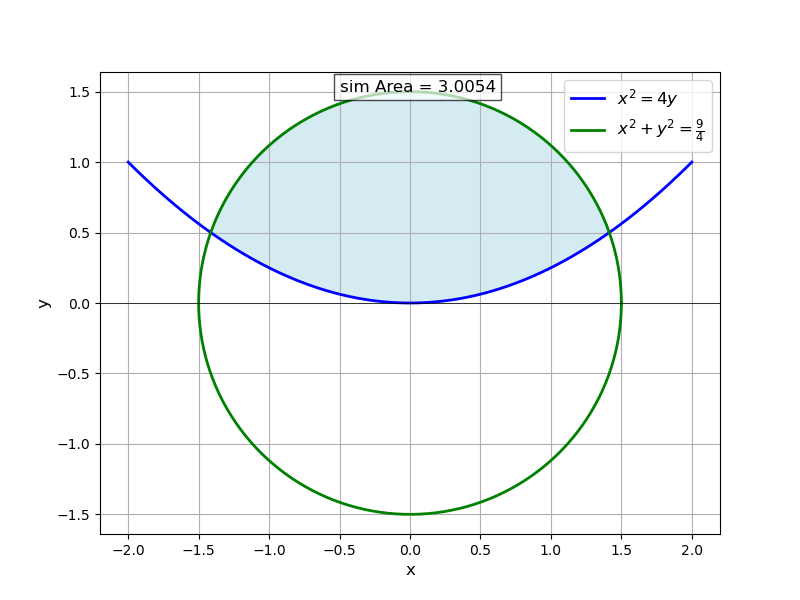
\includegraphics[width=\columnwidth]{figs/Figure_1.png}
	\label{stemplot}
\end{figure}
\end{document}
